\documentclass[10pt,a4paper,twocolumn]{article}
\usepackage[backend=biber,natbib=true,style=numeric,maxnames=50,sorting=none]{biblatex}
\usepackage{amsmath}
\usepackage{float}
\usepackage{authblk}
\usepackage{fancyhdr}
\usepackage{graphicx}
\usepackage[pdfauthor={Tolga Girici and Ahmet Cihat Kazez},
			pdftitle={Clustering-Based Device-to-Device Discovery and Content Delivery in Wireless Networks},
			pdfsubject={The subject is not clear},
			pdfkeywords={Advertisement, caching, content delivery, device‑to‑device communication, discovery, offloading},
			pdfproducer={International Telecommunication Union},
			hidelinks]{hyperref}

\pagestyle{fancy}
\fancyhf{}
\rhead{{\footnotesize ITU Journal on Future and Evolving Technologies, Volume 2 (2021), Issue 2, 31 May 2021}}
\lfoot{© 2021 International Telecommunication Union}
\rfoot{\thepage}

% Keywords command
\providecommand{\keywords}[1]
{	
	\textbf{\textit{Keywords---}} #1
}

\date{}

%%%%% begin editing here %%%%%

% article specific packages
\usepackage{subcaption}
\usepackage{wrapfig}
\usepackage{tikz}
\usetikzlibrary{arrows}
\usetikzlibrary{snakes}
\usetikzlibrary{calc,patterns}

% article bibliography file
\addbibresource{ituJournalPaper.bib}

% title
\title{Clustering-Based Device-to-Device Discovery and Content Delivery in Wireless Networks}

% authors
\author[1,*]{Tolga Girici}
\author[1]{Ahmet Cihat Kazez}

% affiliations and corresponding author
\affil[1]{Electrical and Electronics Engineering, TOBB University of Economics and Technology, Ankara, Turkey}
\affil[*]{\small Corresponding author: Tolga Girici, tgirici@etu.edu.tr}

\def\abstract{\itshape}

\begin{document}

\twocolumn[
\begin{@twocolumnfalse}
	\maketitle
	\hrulefill \\
	\textit{\textbf{Abstract}---}
	\begin{abstract}
		Device-to-device (D2D) cache placement and content delivery is a recent technology that exploits idle memory capacity of mobile devices and promises to fulfill users' content needs with very low delay and without using the scarce cellular network capacity. Recent literature on D2D caching mostly concentrated on optimal cache placement and mostly disregarded the required discovery mechanisms and the accompanying overhead. In this work we propose a clustering-based procedure that is used to cache content at the helper nodes along with advertisement and discovery procedures for content delivery. We implement a Long Term Evolution (LTE)-based simulation setup to evaluate the proposed schemes. Numerical results reveal that the clustering-based user and content discovery significantly improves cellular offloading and reduces the discovery overhead with a minimal sacrifice from delay.
	\end{abstract}
	\bigskip
	\keywords{Advertisement, caching, content delivery, device‑to‑device communication, discovery, offloading}
	\bigskip
	\end{@twocolumnfalse}
]

\section{Introduction} 
\label{sec:intro}
Recent technological improvements have triggered the widespread use of connected devices and caused a dramatic increase in mobile data demand. While meeting this demand service providers must also fulfill users' essential Quality of Service (QoS) requirements such as high data rate and low latency. This exigency is conducive to the birth of new technologies in next generation communication systems, particularly for 5G and beyond. Device-to-device (D2D) communication is one of these technologies which enables direct communication of nearby users without any Base Station (BS) assistance and alleviates load on the Radio Access Network (RAN) and core network. Benefits of D2D may be listed as high spectral efficiency, reduced latency, extended capacity, and improved power efficiency \cite{5GBookAfif}. D2D communication may utilize licensed (in-band) and unlicensed (out-band) spectrum as well. In-band D2D communication has been defined in the 3rd Generation Partnership Project (3GPP) Release 12 and adopted to existing Long Term Evolution (LTE) technology with the name LTE Direct. In the scope of 3GPP Rel. 12 network architecture, discovery procedures, synchronization, authorization, and group operations are standardized \cite{3gpp.23.303}.

Today, as an add-on technology LTE Direct is not prevalent and has limited usage in public services such as health care and security applications. On the other hand, for 5G, D2D communication is one of the innate technologies and leads to several proximity-based services, such as social networking, emergency communication, Internet of Things (IoT) enhancement, commercial and media services \cite{wuwhitepaper}. Cache placement and content delivery are considered vital applications of D2D communication \cite{chiasserini2015content}. Since D2D technology is device-centric and data transmission is exempt from RAN and core network traffic, requested content must be cached by the edge devices beforehand and delivered upon request \cite{Bastug2014LivingontheEdge}.

In the literature there are several studies that investigate  the cache placement and content delivery for D2D based networks with an aim of optimizing throughput, hit rate and delay with effective usage of limited cache capacity of edge devices \cite{chen2017cache, zhang2017user, lin2017extensive, xu2018towards, sun2019cost, sun2020delay, zhang2019d2d, ji2015throughput}.

Widespread adoption of the D2D technology requires efficient, practical, and implementable schemes for cache placement and content discovery, along with new business models \cite{chiasserini2015content}. In the literature, studies on D2D cache placement mostly considered optimization-based approaches that disregarded practicality aspects. Optimization problems are formulated and solved in order to maximize coverage \cite{chen2017cache},  offloading \cite{zhang2017user}, hit ratio \cite{xu2018towards, AnjumCache2019, LinCaching2020, Soleimani2018Caching}, minimize delay \cite{lin2017extensive, sun2020delay} and minimize cost \cite{sun2019cost}, under constraints such as  cache capacity \cite{LinCaching2020}, delay and coverage \cite{Soleimani2018Caching}. An optimal cache placement problem that aims to maximize offloading has been formulated and solved jointly with the D2D link establishment scheme in \cite{ZhaoCaching2018}.

There are also game-theoretic schemes that are proposed to maximize revenue \cite{zhang2019d2d}. An incentive-based game theoretical approach for the cache placement problem is presented in \cite{Zhu2016Incentive}.  Another group of work utilized stochastic geometry, where the distribution of nodes is considered as a spatial random process. The authors in \cite{chen2017optimal, chen2017high,ChenCaching2017, lee2018caching, amer2020optimized} used stochastic geometry and found randomized caching (in some works along with randomized scheduling \cite{chen2017optimal} ) policies in order to maximize throughput. However, these works only reveal some fundamental trade-offs between throughput and node density and do not give the performance in an actual network, as the actual node distribution may not be a Poisson point process. The above works on optimal D2D cache placement are assumed to be implemented in a centralized manner. Moreover, these works did not address user and content discovery, which is an important aspect of D2D communications.

Clustering is an important concept in ad hoc networks. It is used in order to group nearby users into a cluster and designate a cluster head, in order to facilitate distributed network functions. Clustering can be utilized in D2D communications in order to implement practical cache placement and content delivery schemes. In the literature clustering in D2D communications is utilized in order to use some devices as cluster heads (CH) that relay data coming to and from the base station. Clustering methods proposed in \cite{yaacoub2013achieving} and \cite{asadi2017network} are based on  merge and split operations and they can be implemented in a centralized manner. Authors in \cite{doumiati2017framework} proposed a clustering scheme that is within the confines of LTE standards.  Users detect their neighbors and report list of their neighbors to the BS. Then the BS forms clusters based on the neighborhood information. In \cite{zhang2017peer, feng2018resource, yang2018social} the authors propose centralized clustering methods that are based on social as well as physical layer attributes. In \cite{gharbieh2018self} cluster heads are used as relays of scheduling requests in order to alleviate the congestion at the physical random access channel (PRACH). Cluster head selection is randomized and cluster formation is distributed. The work in \cite{gupta2018cluster} utilizes distributed clustering for vehicular networks. In the above-mentioned works, caching was not considered. Recent works such as \cite{swain2020novel} and \cite{asheralieva2020combining} did not consider cache placement, but proposed  clustering schemes based on cached content, as well as social and physical layer attributes.

The above-mentioned works reveal that clustering is a useful technique and it's been utilized for various goals in LTE-based D2D transmission literature.  The authors in \cite{Kazez2019Clustering} were the first ones to jointly address D2D clustering and cache placement. They proposed an algorithm that clusters helper (caching) nodes and then allocates content in each cluster member in a way that maximizes offloading and performs very close to the optimal solution.  However, none of the above-mentioned considered cache placement jointly with the required content/user discovery operations.

A crucial point in D2D communications is the \emph{discovery} operation which might denote device, content, and service discovery. Regardless of the purpose of discovery, these operations cause messaging overhead and interference induces outages in networks with high user density. Therefore, discovery in D2D communication has to be handled wisely \cite{chiasserini2015content}. Discovery operation could be done in a centralized or distributed manner. In the \emph{network-assisted}  discovery, the BS or another centralized entity that possesses the network information provides proximity information, channel state information, resource allocation information to the users. However, it requires network coverage and computational complexity along with the increasing number of users. In the \emph{distributed discovery} , users have to cope with the discovery process on their own, without any external assistance. It does not require network coverage but is ineffective in the resource utilization.

In the literature, several studies cover device and service discovery. Authors have proposed a clustering algorithm and a two-step discovery procedure that aims to reduce signaling overhead and enables simultaneous discovery in \cite{swain2020novel} but cache placement and content delivery issues are foreclosed. In \cite{Gunes_2014} a hybrid scheme has been proposed in D2D, which includes a direct discovery phase and network-assisted data communication phase for proximity services. In the discovery phase, authentication and authorization are provided by the operator initially upon D2D request. The authors also stated that the network-assisted D2D communication phase satisfies users' privacy and security concerns. Another hybrid scheme is presented in \cite{LiDiscovery2018} that aims improvement both in energy consumption and latency compared to direct discovery. In \cite{Prasad2014} an Evolved Packet Core (EPC) assisted discovery approach has been considered, where users activate their D2D capabilities in specific areas after invoked by BS to increase the success rate and energy efficiency. An eNB assisted discovery and D2D link setup procedure is proposed in \cite{Hong_2013} and performance is evaluated in terms of energy consumption and delay. Centralized and semi-centralized D2D discovery algorithms are introduced and compared in terms of required time slots to discover all new D2D pairs in the cell in \cite{Thanos_2013}. In \cite{ParkDiscovery2017} two device discovery schemes have been proposed for centralized and autonomous D2D networks that aim to reduce power consumption and signaling overhead. The authors also claim that the proposed schemes are applicable for cache enabled D2D networks. Contrary, in \cite{Xu2018Discovery} users can discover each other not only directly but also via forwarding nodes. To overcome excessive energy consumption in direct discovery procedures of Wi-Fi Direct Technology, authors proposed an LTE network assisted peer discovery \cite{PyattaevWiFiDirectDiscoveryLTE}.

As mentioned formerly, LTE Direct is the only technology that enables D2D communication in the cellular spectrum (also known as in-band D2D). Two discovery schemes have been defined in the technical specification documents of the LTE Direct \cite{TSLTEDirect}. In the Network Assisted scheme, User Equipments (UEs) that have been registered for D2D communication are warned about proximate devices. On the other hand, in the Direct Discovery, UEs send discovery beacons to discover other UE and proximity services in an unabetted way.

\subsection{Contributions}
\label{ssec:ssec1.2}
Apart from the existing literature, in this paper a comprehensive study on D2D communication, which covers most of the key aspects of D2D technology such as user clustering, cache placement, discovery, advertisement, and resource utilization are presented.

At first, we are reminded of the previously proposed Distance Based Clustering Algorithm (DBCA) and Hierarchical Caching Algorithm (HCA) \cite{Kazez2019Clustering, KazezMobility2019}. DBCA aims to form maximal cliques and boost cooperation among Helper Users (HUs). Moreover, HCA provides effective usage of users' limited cache capacity and maximizes the network's average offloading. Furthermore, we propose Advertisement Based (ABD2D) and Discovery Based (DBD2D) D2D user/ content discovery  procedures to complement the DBCA and HCA. These schemes aim to advertise cached content by the clusters and discovery of cached content by Ordinary Users (OUs), respectively.

A model network comprises mobile cellular users where some of them (HUs) are cache enabled and able to create clusters in order to make cache placement and content discovery more efficient, in terms of offloading and control messaging overhead. Clustering and cache placement algorithms are applied consecutively before the proposed advertisement and discovery procedures. This is the first work that addresses the D2D-based distributed cache placement and content delivery along with the critical components of device discovery and content advertisement. We have implemented an LTE-based simulation setup and  analyzed the performance of proposed procedures in terms of average offloading and messaging overhead against a varying number of Discovery Resource Blocks (RBs), Helper Users(HUs), Ordinary Users (OUs) and Signal to Interference Noise Ratio (SINR) threshold. Results are presented, discussed and highlighted in Section \ref{sec:sec6}.

\section{System Model}
\label{sec:sec2}
We consider a simplex content delivery procedure between cellular users where HUs provide content to OUs upon request.  A model network consists of a Base Station (BS) placed at the center of a circular area and all users are randomly distributed. Users are categorized into three groups: 

\begin{itemize}
	\item \textbf{Helper Users (HUs)} are able to cache content and provide them to the OUs via D2D links upon request. HUs are also able to form clusters with the help of the BS and manage intra-cluster cache placement in a hierarchical structure.  
	
	\item \textbf{Isolated Helper Users (IHUs)} have the same role and abilities as HUs but at a certain time slot they have not been able to join any cluster and thus stay alone. IHUs cache and serve content individually. Since all HUs are mobile, relative positions are time-varying. Therefore, being isolated might be thought of as a transient state.
	
	\item \textbf{Ordinary Users (OUs)} are not cache enabled and acquire available content from HUs via D2D links. OUs request desired content from BS if they cannot establish D2D links via the proposed procedures.
\end{itemize}

In the model network, all users are moving according to the Random Direction Mobility Model (RDMM) \cite{Waqas2020Mobility}. In RDMM users move towards a random direction with a random speed until they reach the boundary of the area. At the edge of the boundary users bounce back to the area and keep moving until the end of the simulation. Since realizing the cell borders are unlikely, bouncing users can be interpreted as newcomers to the cell. Fig. \ref{fig:topology} illustrates the system model.

\begin{figure}[htb]
	\centering
	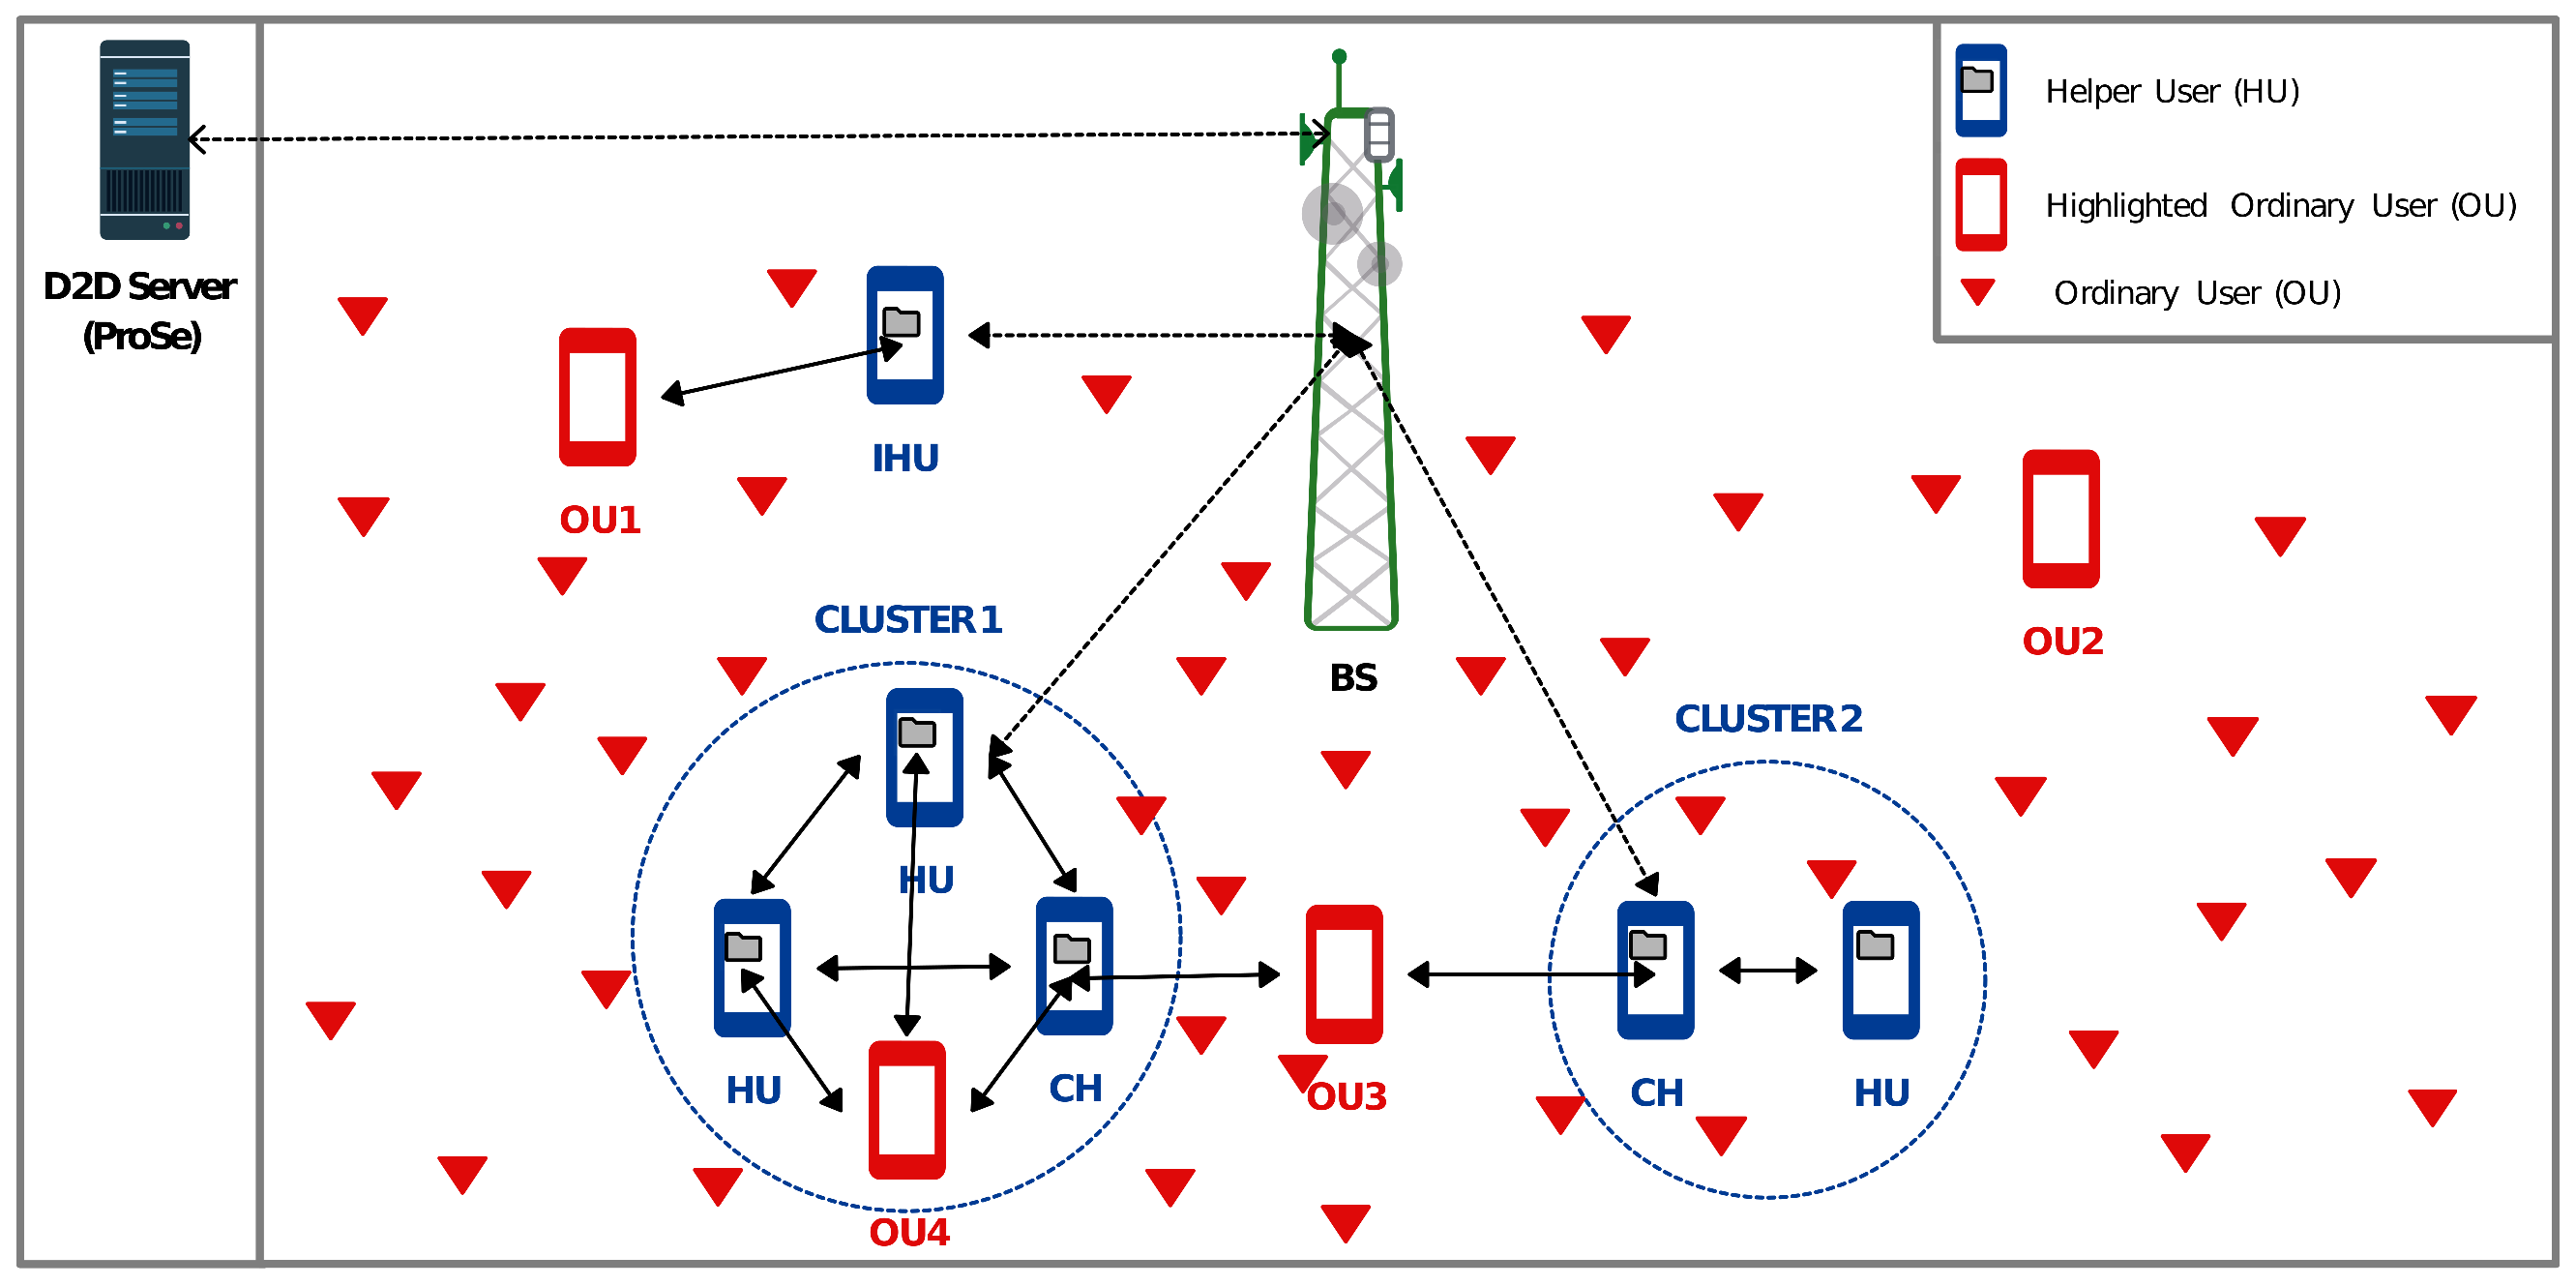
\includegraphics[width=\columnwidth]{topology.eps}
	\caption{Illustration of Network Topology}
	\label{fig:topology}
\end{figure}

Content set ${1,2,...,C}$ is bounded and HUs have limited cache capacity ($C_c$) which	necessitates an excogitated cache placement approach. Each content is assumed to be of equal size. Content popularity among users are uniform, Zipf distributed at each user and assumed to be known by all users in the network. According to the Zipf's Law, out of a content set with $C$ elements popularity of the content of rank $n$ is defined as \cite{ZipfDist};

\begin{equation}\label{eq:zipf}
	f(n:\alpha,C)=\frac{\frac{1}{n^{\alpha}}}{\sum_{c=1}^{C}(\frac{1}{c^{\alpha}})}
\end{equation}

Where $\alpha$ is the skewness exponent of the Zipf distribution. Bigger $\alpha$ reveals the domination of the most popular content, while on the other hand smaller $\alpha$ induce to a more uniform-likely distribution. $C$ is the size of the content set and $n$ is the rank of the content where $n=1$ stands for the most popular content of the set.

For successful content delivery, in addition to content availability, some other conditions must be met. First of all, users must meet the SINR threshold constraint to exchange discovery/advertisement beacons. Since the number of dedicated RBs for discovery and advertisement procedures are limited and randomly selected by users, interference and collisions are inevitable. Without exception, HUs and OUs, which are exposed to interference, are unable to establish D2D links in an Awareness Zone (AZ), cannot receive and transmit content in the Delivery Zone (DZ) and cannot make any contribution to offloading sequentially. On the other hand, if discovery is successful, enough resources are assumed to exist and content transmission is assumed to be successful. LTE physical layer and channel models \cite{KyostiWinner} are adopted in the simulations.

In Fig. \ref{fig:topology} the network topology is illustrated. Solid lines with solid arrows indicate D2D communication. D2D links between HUs are required for intra-cluster operations. Four of the OUs are highlighted to depict some particular cases. 1) OU1 is not close enough to a CH and only a nearby IHU serves requested content. 2) OU2 neither has a CH nor an IHU in its D2D range for the corresponding time slot. 3) OU3 is in coverage of two CHs. 4) Similarly OU4 has a link to a CH and is able to exploit content from cluster members. Moreover, dashed lines with solid arrows indicate a cellular link and a dashed line with the thin arrow indicates the control plane interface between the BS and ProSe Server. The role of these links is described in the following sections.


\section{Offloading Formulation}
\label{sec:sec3}

For the sake of completeness, the problem of offloading maximization, originally formulated in \cite{Kazez2019Clustering} is given in \ref{eq:optim}. We assume that there are $U$ ordinary users, $H$ helper users and $C$ contents.  Here $p_{uc}$ is popularity of content $c$ for OU $u$, which is Zipf distributed and uniform among all OUs. Decision variable $y_{huc}$ takes binary values and indicates delivery of content $c$ to OU $u$ from HU $h$. Parameter $s_c$ stands for content size. Another binary variable $x_{hc}$ indicates that content $c$ is cached by helper $h$. The sum of $x_{hc}$ along $h$ is limited to cache capacity $C_c$. Moreover, $a_{hu}$ stands for the SINR based D2D eligibility between HU $h$ and user $u$. Accordingly, \ref{eq:neighbor} enforces that an OU $u$ can receive help from HU $h$, in terms of content $c$, only if HU $h$ caches that content and HU/OU meets the SINR threshold condition.

\begin{equation}\label{eq:optim}
	Offloading= \left\{\sum_{u=1}^{U}\sum_{c=1}^{C}p_{uc}\sum_{h=1}^{H}y_{huc}s_c\right\}
\end{equation}\\
s.t.
\begin{equation}
	\sum_{c=1}^{C} x_{hc}s_c \leq C_c , \forall h=1,\ldots,H \label{eq:cachecap}\\
\end{equation}

\begin{equation}
	\sum_{h=1}^{H}y_{huc} \leq 1, \forall u=1,\ldots,U, c=1,\ldots,C \label{eq:singlehelper} \\
\end{equation}

\begin{equation}
	\begin{aligned}
		y_{huc} \leq a_{hu}x_{hc}, \forall u=1, &\ldots, U,\\
		c=1,&\ldots,C,\\ 
		h=1,&\ldots,H \label{eq:neighbor}
	\end{aligned}
\end{equation}

The formulation described above maximizes offloading for a given (static) network topology and disregards mobility. Besides, it assumes perfect user/content discovery. For a mobile network, this optimization problem has to be solved periodically with sufficient frequency and it has a prohibitive complexity.

\section{Clustering and Cache Placement Operations}
\label{sec:sec4}
Proposed ABD2D and DBD2D procedures are envisaged to work in conjunction with DBCA and HCA that were originally proposed in \cite{Kazez2019Clustering}. Therefore, in the scope of this paper, we evaluate the performance of these algorithms once again and investigate the adaptation of pre-proposed algorithms and currently proposed procedures as a whole. Shortened descriptions of the algorithms are given below.

\textbf{Distance Based Clustering Algorithm (DBCA)} aims to cluster nearby HUs and pave the way for facilitating collaboration among cache enabled devices by providing content diversity. In our clustering approach: 1) All cluster members are close enough to establish direct D2D links between each other, this enables intra-cluster coordination. 2) Cluster members act in a hierarchical structure, the HU that has the most number of OUs in its D2D range is designated as the Cluster Head (CH). Cache placement is managed by the CH and cache capacity of the cluster is considered as a whole. 3) Each HU can be a member of only one cluster; this constraint prevents conflicts in caching. We assume that the clustering operation is managed by the D2D ProSe server, which receives the neighborhood information from HUs as input, as in \cite{doumiati2017framework}.

Cache placement operation is managed by the CH relying on the \textbf{Hierachical Caching Algoritm (HCA)} \cite{Kazez2019Clustering}. This algorithm is managed by the head of each cluster. The algorithm accepts cluster information, content popularity ($p_{uc}$), number of contents ($C$) and cache capacity of HUs ($C_c$) as inputs. For each cluster, initially total cache capacity is calculated and cluster level caching layout is determined as to how many copies of each content will be cached. Then HU-level cache placement is determined according to the cluster's hierarchical order. Resultant cache placement may include duplicate copies of popular content in multiple cluster members, or some content may not be cached at all. As an exception, HUs that are not members of any cluster are classified as isolated HUs (IHU), cache the most popular content and serve OUs individually. Content to be cached is requested from the BS.

In this work, we assume that clustering and cache placement procedures are repeated periodically in order to cope with mobility. The robustness of the algorithm pair (DBCA and HCA) against mobility was investigated in \cite{KazezMobility2019}. A reasonable update period of 10-15 seconds resulted in a small performance loss (around $ 4-5\%$). 


\section{Proposed Advertisement and Discovery Procedures}
\label{sec:sec5}

As mentioned in Section  \ref{sec:intro}, previous studies on D2D caching (including \cite{Kazez2019Clustering}) mainly overlooked D2D user and content discovery. In this section, the proposed  content delivery procedures, namely ABD2D and DBD2D are  presented. For both, it is assumed that clustering and cache placement operations are applied beforehand.

The ABD2D procedure, illustrated in Fig. \ref{fig:ABD2D}  is initialized by the advertisement beacons broadcast by CHs and IHUs. These beacons first and foremost include cluster information and available content. Advertisement beacons are transmitted using the limited number of allocated and randomly selected discovery Resource Blocks (RB). Each advertisement beacon may not be received by UEs due to the short-range of D2D communication and collisions. Simultaneous access to a channel causes interference and if instantaneous SINR cannot exceed the determined SINR threshold, a D2D link cannot be established between meddling users at the corresponding RB. OUs reply to advertisement beacons if any available content is required. This reply beacon includes measured SINR information to make a channel state estimation while scheduling D2D communication.

In the next step, the CH informs the corresponding cluster member HU that cached requested content and  informs BS about D2D link. In order to schedule the D2D transmission BS needs instant topology and D2D link information. This information is kept on the D2D Server (ProSe) and provided upon request. Then BS schedules D2D communication with a control message  that includes transmission channel, transmit power and synchronization information. For the sake of simplicity and in order to avoid overhead, only the CHs communicate with the BS and they need to inform the HUs about the schedule. At the end of the ABD2D procedure, handshake occurs between a D2D pair and then the requested content is provided. The main advantage of ABD2D is the clustering, wherein only the CH communicates with OUs and the BS, which reduces the collisions and overhead.

\begin{figure*}
	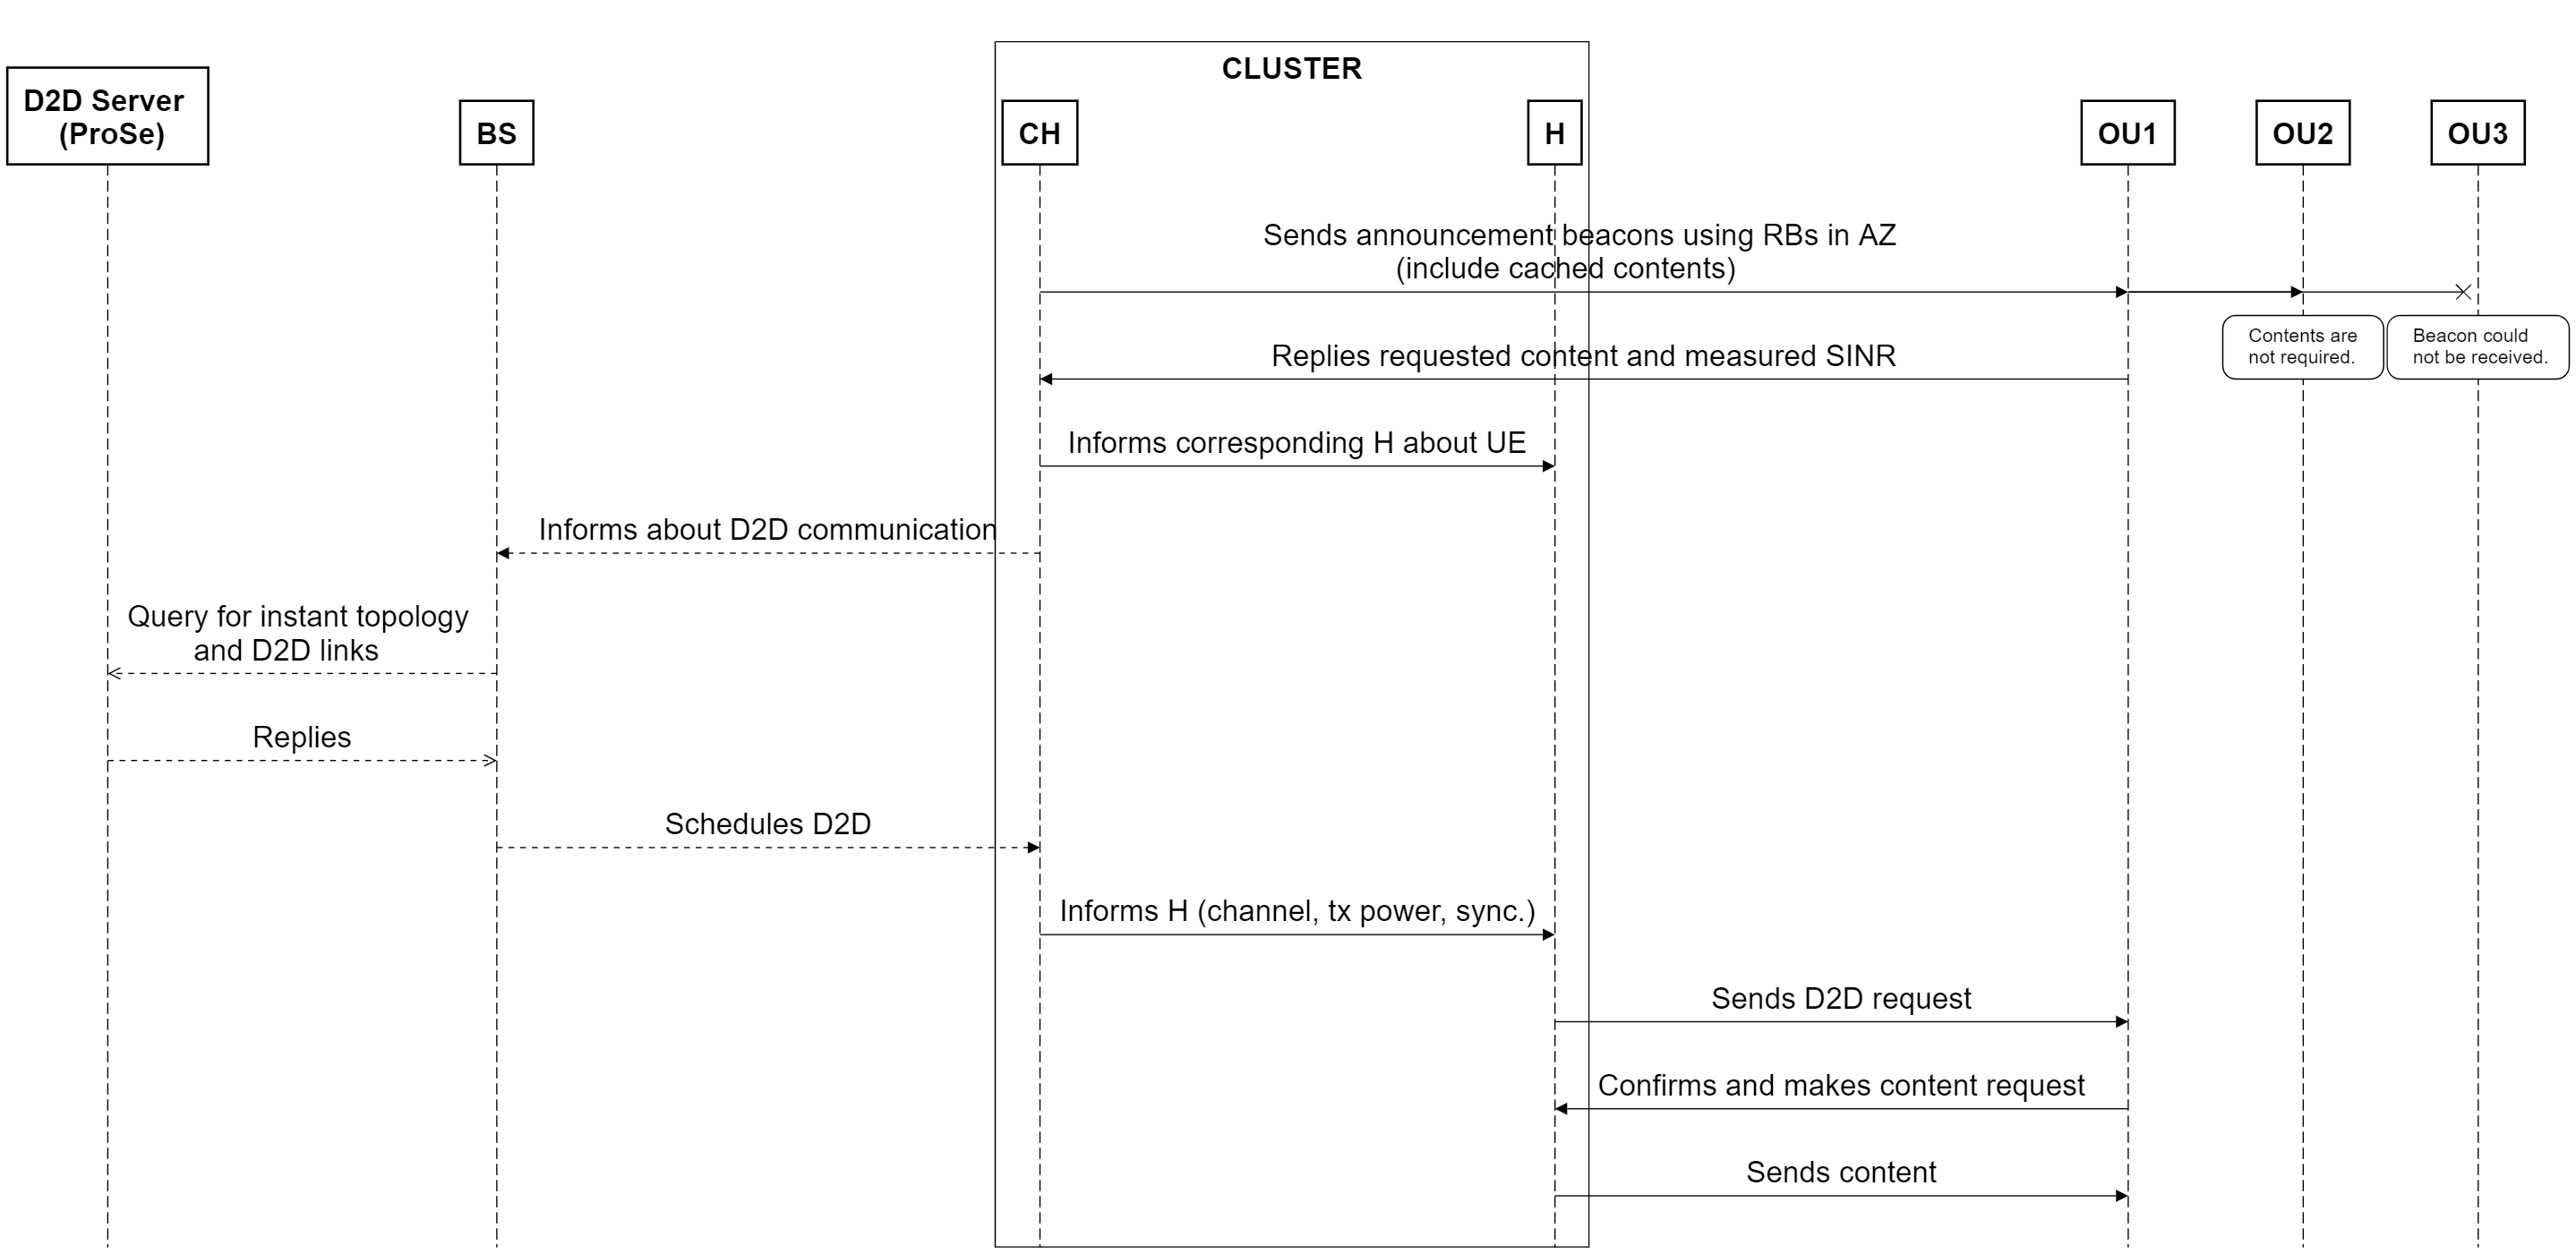
\includegraphics[width=\textwidth]{ABD2D.png}
	\caption{Flow diagram of the ABD2D communication procedure}
	\label{fig:ABD2D}
\end{figure*}

Initialization of the DBD2D procedure, illustrated in Fig. \ref{fig:DBD2D}, is different from ABD2D but the rest is quite similar. DBD2D is triggered by discovery beacons broadcast by OUs that request content. These beacons include desired content and are received by CHs and IHUs. Since only the CHs are responsible for intra-cluster operations and handles the BS interface, cluster member HUs do not listen to discovery channels. Resource allocation and usage are clarified in detail in the following sections.
For both procedures, illustrated in Fig. \ref{fig:ABD2D} and Fig. \ref{fig:DBD2D}, solid lines indicate D2D communication, dashed lines with solid arrows indicate a cellular link and dashed lines with thin arrows indicate a control plane interface between the BS and ProSe Server, similar to the PC4 interface in the LTE architecture. 

\begin{figure*}
	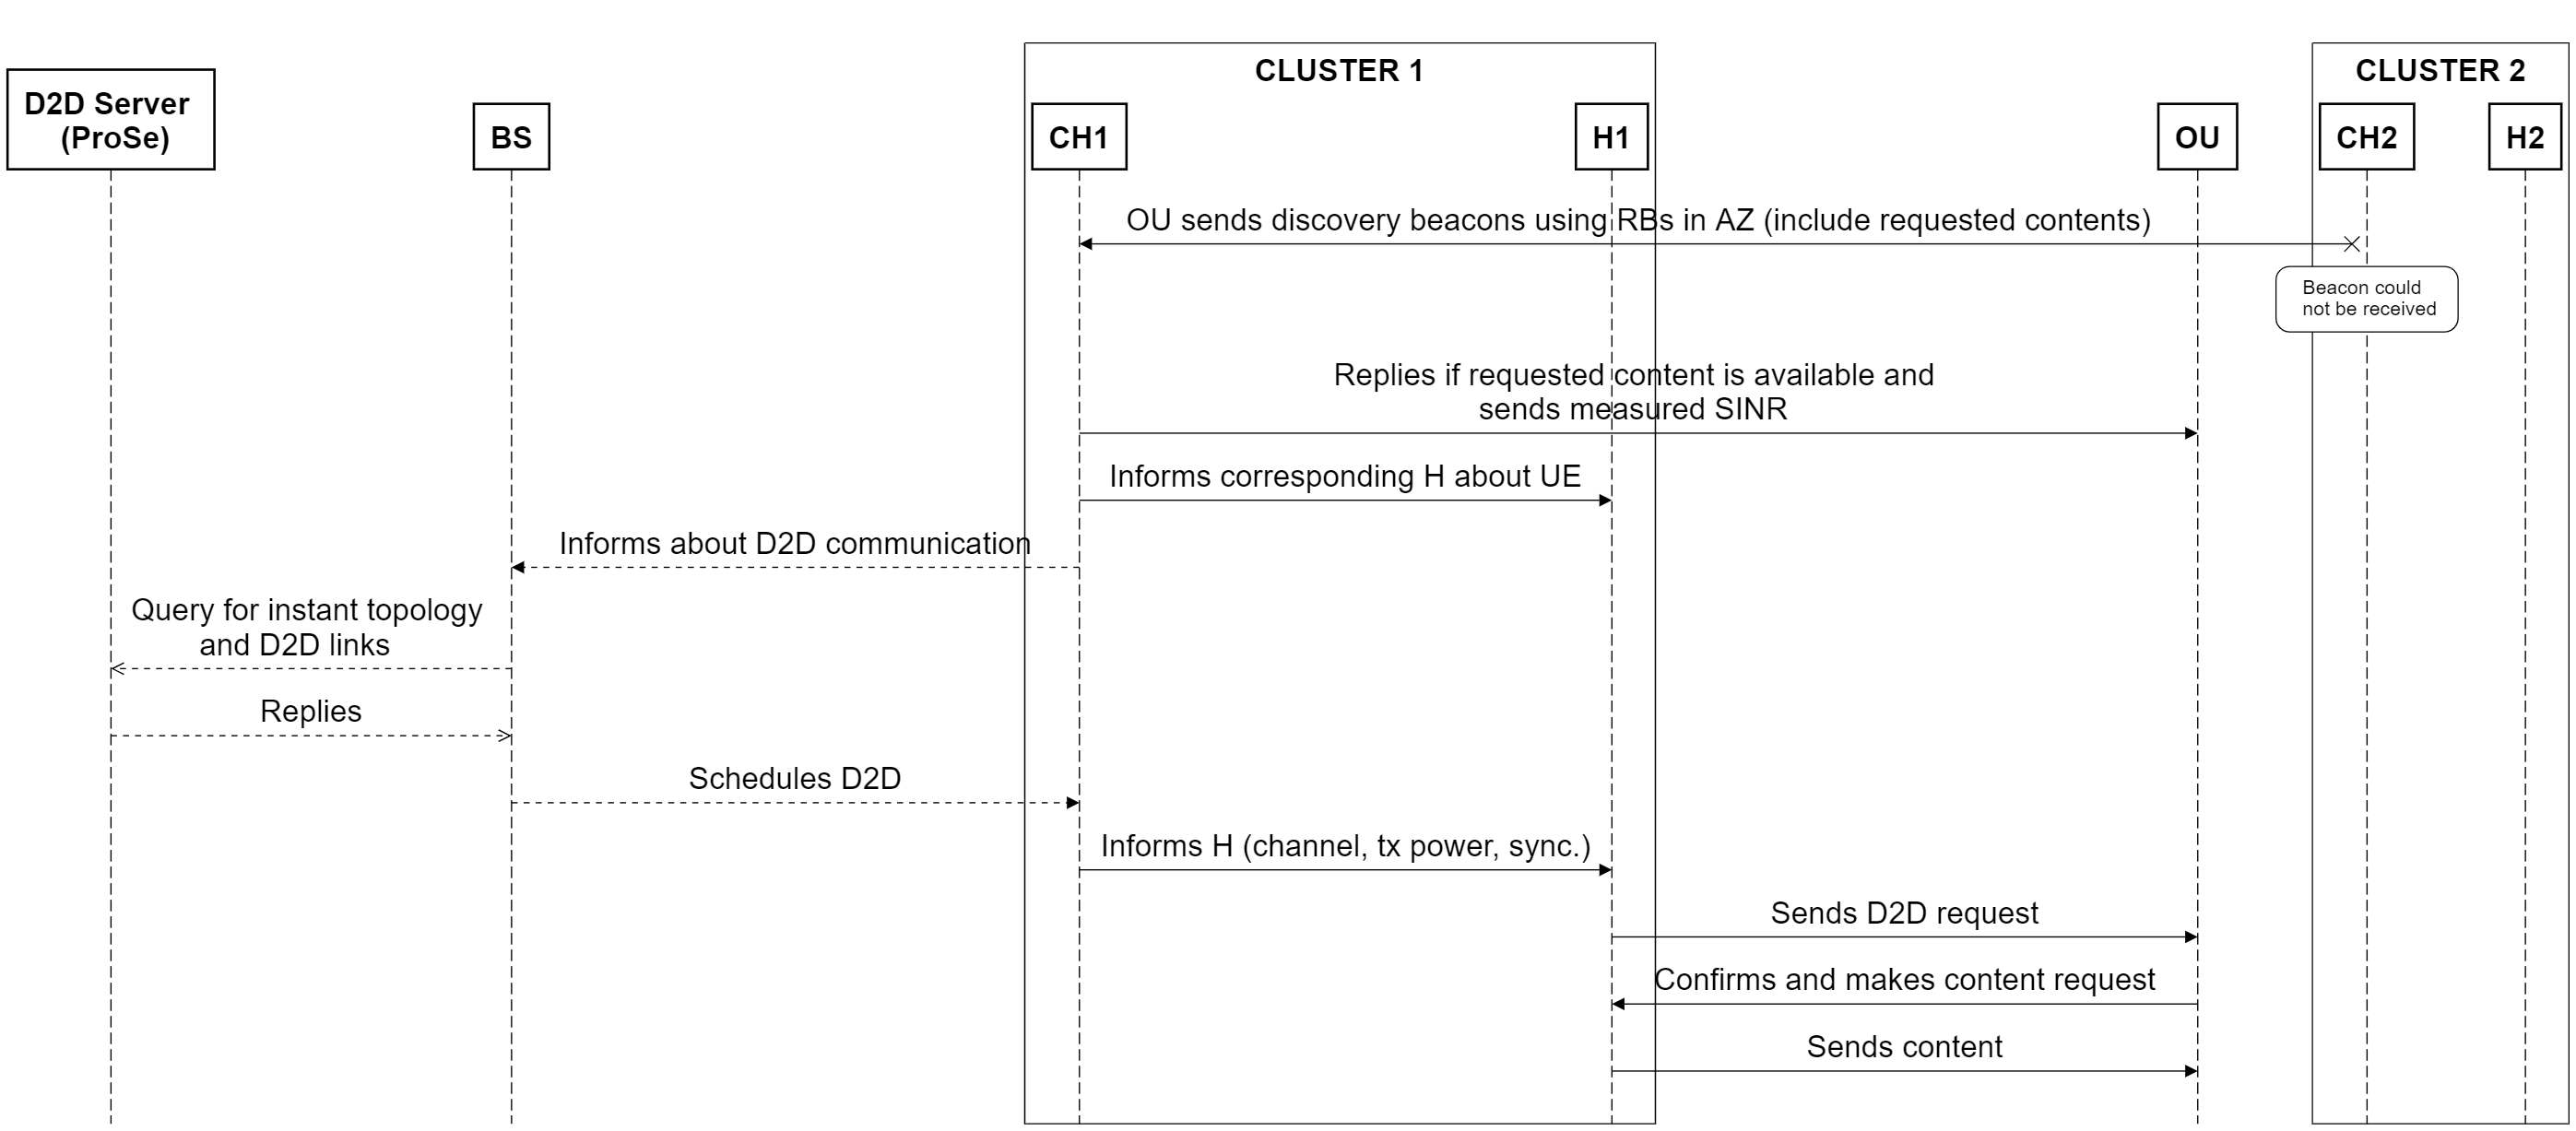
\includegraphics[width=\textwidth]{DBD2D.png}
	\caption{Flow diagram of the DBD2D communication procedure}
	\label{fig:DBD2D}
\end{figure*}

\section{Resource Allocation and Access Model}

In the model network, transmission and reception occur in a half duplex manner for both of the proposed procedures. This means, while OUs are transmitting discovery beacons, CHs and IHUs stay in the receiving state and vice versa. For this purpose, time is divided into segments and each segment includes a varying number of time slots where a time slot is the smallest piece of time. All of the steps defined in Fig. \ref{fig:ABD2D} and Fig. \ref{fig:DBD2D} take place in the predefined time allotment sequentially.

Resource allocation, in the time and frequency domain, has been managed by the core network on a not UE-specific basis, and users are informed about allocations via System Information Block (SIB) content similar to LTE \cite{36843}. Such an approach provides a reduction in the computational complexity and signaling overhead. On the other hand, this may cause ineffective usage of resources because of autonomous access to resources.

\begin{figure} [htb]
	\centering
	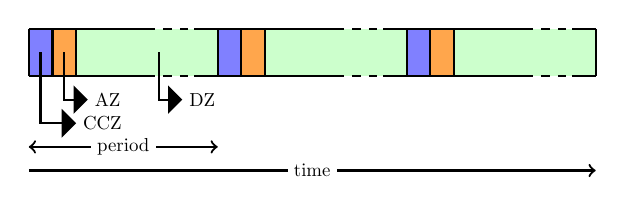
\begin{tikzpicture}[thick,fill opacity=1,scale=0.6, every node/.style={scale=0.68}]
		
		
		\fill[green!20] (0.5,0) rectangle (11.5,1);
		\fill[orange!70] (0,0) rectangle (0.5,1);
		\fill[orange!70] (4,0) rectangle (4.5,1);
		\fill[orange!70] (8,0) rectangle (8.5,1);
		\fill[blue!50] (7.5,0) rectangle (8,1);
		\fill[blue!50] (-0.5,0) rectangle (0,1);
		\fill[blue!50] (3.5,0) rectangle (4,1);
		
		\draw[solid] (-0.5,0) -- (2,0); \draw[solid] (3,0) -- (4,0); \draw[dashed] (2,0) -- (3,0);
		\draw[solid] (-0.5,1) -- (2,1); \draw[solid] (3,1) -- (4,1); \draw[dashed] (2,1) -- (3,1);
		
		
		\draw[solid] (4,0) -- (6,0); \draw[solid] (7,0) -- (8,0); \draw[dashed] (6,0) -- (7,0);
		\draw[solid] (4,1) -- (6,1); \draw[solid] (7,1) -- (8,1); \draw[dashed] (6,1) -- (7,1);
		\draw[solid] (3.5,0) -- (3.5,1); 
		\draw[solid] (7.5,0) -- (7.5,1); 
		
		
		\draw[solid] (8,0) -- (10,0); \draw[solid] (11,0) -- (11.5,0); \draw[dashed] (10,0) -- (11,0);
		\draw[solid] (8,1) -- (10,1); \draw[solid] (11,1) -- (11.5,1); \draw[dashed] (10,1) -- (11,1);
		
		\draw[solid] (-0.5,0) -- (-0.5,1);\draw[solid] (0,0) -- (0,1);\draw[solid] (0.5,0) -- (0.5,1); \draw[solid] (4,0) -- (4,1); \draw[solid] (4.5,0) -- (4.5,1);\draw[solid] (8,0) -- (8,1);\draw[solid] (8.5,0) -- (8.5,1);\draw[solid] (11.5,0) -- (11.5,1);
		
		\draw[->] (-0.5,-2) -- (11.5,-2) node[midway,fill=white, text centered]{time};
		\draw[<->] (-0.5,-1.5) -- (3.5,-1.5) node[midway,fill=white, text centered]{period};
		\draw[-triangle 90] (0.25,0.5) |- (0.75,-0.5) node[right,fill=white, text centered]{AZ};
		\draw[-triangle 90] (-0.25,0.5) |- (0.5,-1) node[right,fill=white, text centered]{CCZ};
		\draw[-triangle 90] (2.25,0.5) |- (2.75,-0.5) node[right,fill=white, text centered]{DZ};
		
	\end{tikzpicture}
	\caption{Clustering and Cache Placement Zone (CCZ), Access Zone (AZ) and Delivery Zone (DZ) - Periodic allocation}
	\label{fig:AZAllocation}
\end{figure} 

In each period, three discrete operations are handled as shown in Fig. \ref{fig:AZAllocation}. In the beginning, in Clustering and Cache Placement Zone (CCZ) DBCA and HCA occurs according to the procedures described in Section \ref{sec:sec4}. Clustering is periodically maintained by the ProSe server in the CCZ, in order to adapt to mobility.  Then, in the Awareness Zone (AZ), ABD2D and DBD2D procedures are applied. Lastly, in the Delivery Zone (DZ) content delivery via D2D links takes place.  We assume that the length of a period is constant and dedicated durations are long enough to complete assigned tasks for CCZ \& DZ. As mentioned earlier, all users are mobile and keep moving according to the RDMM during the entire period. Therefore, we also assume that cluster structure is conserved between two consecutive CCZs.

The resource allocation scheme covers only the ABD2D and DBD2D procedures. Thus the longest chunk of the slotted time assumption is the Awareness Zone (AZ) in the scope of this research. It is assumed that an AZ is long enough to complete a DBD2D or ABD2D procedure. During an AZ, UEs that are not able to discover either a CH or an IHU, request the desired content from BS (eNB for LTE).
Each AZ is $2\times N+T$ ms long and composed of three partitions. The first and third partitions are $N$ ms long and reserved for sidelink communication between nearby devices which is similar to the PC5 interface in the LTE architecture. The second partition is held for intra-cluster operations and core network communication of CHs and IHUs. Resource allocation is omitted for the second partition of AZs since IHUs do not occupy RBs and relatively many RBs are allocated for cluster member HUs. (Fig. \ref{fig:TBTahsis})

MP and RP are divided into 1ms length time slots as shown in Fig. \ref{TByapısı} and each time slot consists of 25 resource blocks (RBs). 10 of these RBs are eligible to be used for discovery and advertisement purposes. It is assumed that each RB has a $180$ kHz bandwidth and consists of $12$ subcarriers similar to the LTE. In a non-UE specific based resource allocation scheme users randomly select a time slot and an RB in every MP. The random access to RBs approach is defined in LTE technical reports as Type-1 \cite{36877}. During an MP, $K^{MP}_{i,j}$ indicates that user $K$ sends discovery/advertisement beacons in the $i_{th}$ time slot using $j_{th}$ RB.

In the case of multiple access attempts for an RB, interference at the receiver is inevitable. If the SINR value at the receiver does not exceed the required threshold for any user, the corresponding advertisement/discovery message cannot be successfully received. As an outcome, overlapped users encounter outage, are unable to create D2D links and cannot make a contribution to the offloading. On the other hand, if the SINR value meets the threshold for a user, the corresponding user occupies the RB during the entire AZ and gets a response in the same time slot and over the same RB during the following RP. The SINR threshold depends on the modulation and coding rate \cite{ChiumentoSINR}
\begin{figure} [!htb]
	\centering
	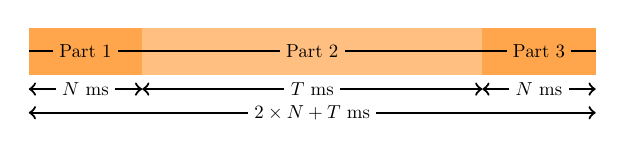
\begin{tikzpicture}[thick,fill opacity=1,scale=0.6, every node/.style={scale=0.68}]
		
		
		
		\fill[orange!70] (0,0) rectangle (2.4,1);
		\fill[orange!50] (2.4,0) rectangle (9.6,1);
		\fill[orange!70] (9.6,0) rectangle (12,1);
		\draw[] (0,.5) -- (2.4,.5) node[midway,fill=orange!70, text centered]{Part 1};
		\draw[] (2.4,.5) -- (9.6,.5) node[midway,fill=orange!50, text centered]{Part 2};
		\draw[] (9.6,.5) -- (12,.5) node[midway,fill=orange!70, text centered]{Part 3};
		\draw[<->] (0,-0.3) -- (2.4,-0.3) node[midway,fill=white, text centered]{$N$ ms};
		\draw[<->] (2.4,-0.3) -- (9.6,-0.3) node[midway,fill=white, text centered]{$T$ ms};
		\draw[<->] (9.6,-0.3) -- (12,-0.3) node[midway,fill=white, text centered]{$N$ ms};
		\draw[<->] (0,-0.8) -- (12,-0.8) node[midway,fill=white, text centered]{$2\times N+T$ ms};
		
		
	\end{tikzpicture}
	\caption{Access Zone (AZ) Structure}
	\label{fig:TBTahsis}
\end{figure}

The first half of the partitions (1 and 3) is used for transmitting discovery/advertisement beacons and called a Messaging Period (MP). On the other hand, the second half is called a Reply Period (RP) and used to reply to advertisement/discovery messages. It is assumed that all users stay in the cellular network coverage during the simulations. Therefore, the time synchronization of users is provided by the network.

\begin{figure}
	\centering
	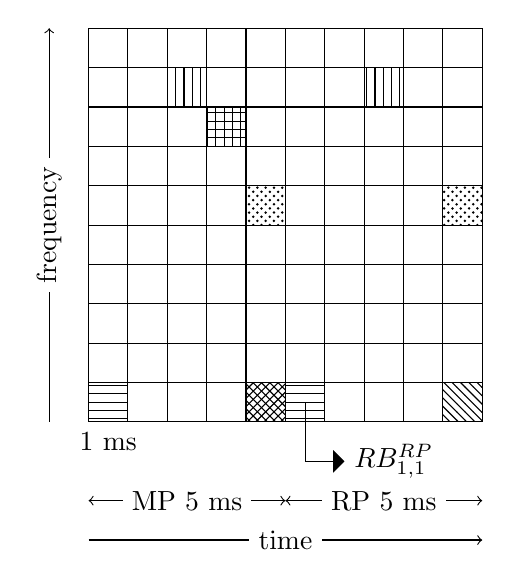
\begin{tikzpicture}
		[box/.style={rectangle,draw=black, minimum size=0.5cm},]
		\foreach \x in {0,0.5,...,4.5}{
			\foreach \y in {0,0.5,...,4.5}
			\node[box] at (\x,\y){};
		}
		\node[box,pattern=vertical lines] at (1,4){};  
		\node[box,pattern=crosshatch dots] at (2,2.5){};  
		\node[box,pattern=horizontal lines] at (0,0){};  
		\node[box,pattern=north west lines] at (2,0){};  
		\node[box,text=white,pattern=north east lines] at (2,0){};  
		\node[box,pattern=grid] at (1.5,3.5){};  
		
		
		\node[box,pattern=vertical lines] at (3.5,4){};  
		\node[box,pattern=crosshatch dots] at (4.5,2.5){};  
		\node[box,pattern=horizontal lines] at (2.5,0){};  
		\node[box,pattern=north west lines] at (4.5,0){};  
		
		
		\draw[<->] (-0.25,-0.5) -- (0.25,-0.5) node[midway,fill=white, text centered]{1 ms};
		\draw[<->] (-0.25,-1.25) -- (2.25,-1.25) node[midway,fill=white, text centered]{MP 5 ms};
		\draw[<->] (2.25,-1.25) -- (4.75,-1.25) node[midway,fill=white, text centered]{RP 5 ms};
		\draw[->] (-0.25,-1.75) -- (4.75,-1.75) node[midway,fill=white, text centered]{time};
		\draw[->] (-0.75,-0.25) -- (-0.75,4.75) node[midway,fill=white, text centered,,rotate=90]{frequency};
		
		\draw[-triangle 90] (2.5,0) |- (3,-0.75) node[right,fill=white, text centered]{$RB^{RP}_{1,1}$};
		
	\end{tikzpicture}
	\caption{Illustration of AZ Part 1 for N=10 ms}
	\label{TByapısı}
\end{figure}

For D2D links Winner B1 Line of Sight (LOS) pathloss model \ref{eq:ploss} is used which is also considered in technical reports prepared by 3GPP for the case of outdoor users \cite{KyostiWinner}.

\begin{multline}
	\label{eq:ploss}
	PL_{HU,OU} = 40\log_{10}\left(d_{HU,OU}\right)+2.7\log_{10}\left(f_{c}/5\right)\\ -17.3\log_{10}\left(h_{HU}\right)-17.3\log_{10}\left(h_{OU}\right)+9.45\\
\end{multline}

As mentioned beforehand, when a discovery or advertisement beacon is successfully received, the corresponding response beacon is sent in the same time slot and over the same RB in the RP. Thus, randomness in the RB selection is avoided and successful delivery of the response message is ensured. In Fig. \ref{TByapısı} the structure of an AZ and some particular cases are illustrated.


\begin{itemize}
	\item  Discovery/advertisement beacon transmitted over $RB^{MP}_{1,1}$ is indicated by horizontal lines and reply to this beacon is transmitted via $RB^{RP}_{1,1}$. Similarly, beacons which are indicated by vertical lines $RB^{MP}_{3,9}$ and dots $RB^{MP}_{5,6}$ also received successfully since these RBs are not selected by any other user and replied over the corresponding RBs in RP. 
	\item $RB^{MP}_{4,8}$ is selected by two users indicated by horizontal and vertical lines. As mentioned previously, this overlap causes an interference at the receiver. Since none of the users fulfill the SINR threshold condition, a reply message is not sent in the RP.
	\item Another particular case for multiple access to the same RB occurs at $RB^{MP}_{1,5}$. This time, the SINR threshold condition is fulfilled by one of the users and a reply is sent over $RB^{RP}_{1,5}$.
\end{itemize}

Moreover, in D2D communication users aim to be aware of each other in an extended range. This might be possible with increasing the transmission power but in dense networks with limited spectrum allocation, this causes interference, outage, and drains the battery. Therefore, similar to the LTE D2D technology, it is assumed that all users have fixed (23 dBm, 200 mW) transmission power \cite{36877}.

In LTE Direct, fixed output power of user equipment prevents usage of Orthogonal Frequency Division Multiple Access (OFDMA). Therefore, the Single Carrier Frequency Division Multiple Access (SC-FDMA) technique is used for uplink to avoid a high Peak-to-Average Power Ratio (PAPR). On the other hand, the OFDMA technique is used for the downlink which provides better spectral efficiency compared to SC-FDMA.

In the proposed network model, the discovery beacon of an OU might be received by multiple CHs or IHUs for DBD2D. Similarly, the advertisement beacon of a CH or IHU also might be received by multiple OUs in ABD2D. In such cases sending reply beacons using the same RB is not possible because SC-FDMA does not allow multiple access to an RB. Since nearby users will attempt to access a common RB with similar output power levels (low PAPR is ensured) without loss of generality we may assume the use of OFDMA which enables the use of subcarriers by different devices \cite{BerardinelliOFDMAvsSCFDMA}. 


\section{Simulation Results}
\label{sec:sec6}

In this section performance evaluation of proposed ABD2D and DBD2D procedures are presented. Number of required control messages for unit offloading and average amount of offloading (number of contents delivered using D2D transmissions) are considered as key performance metrics and investigated against a varying number of HUs, OUs, SINR threshold and allocated MP length for discovery and advertisement. Simulations are performed in MATLAB, for the parameters in Table \ref{table:simparameters}.

\begin{table}[!htb]
	\small
	\centering
	\caption{Simulation parameters}\label{table:simparameters}
	\begin{tabular}{|c|c|}
		\hline
		\textbf{Parameter} & \textbf{Value} \\\hline
		Number of OUs & [100,250,\textbf{400},550,700] \\\hline
		Number of HUs & [30,45,\textbf{60},75,90] \\\hline
		MP duration  & [1,\textbf{2},3,4,5,10,15,20] ms \\\hline
		SINR threshold & [-10,-5,\textbf{0},5,10,15,20] dB \\\hline
		Zipf dist. skewness ($\alpha$)  &  0.6 \\\hline
		Number of contents ($C$) & 20 \\\hline
		Cache capacity ($C_c$) & 4 units \\\hline
		Content size ($s_c$) & 1 unit \\\hline
		Number of random seeds & 100 \\\hline
		Simulation duration & $100\times$period \\\hline
		Period duration & 2 s \\\hline
		Radius of cellular area & 250 m \\\hline
		Mobility model  & RDMM \\\hline
		Max speed of users  & 3 m/s \\\hline
		Transmission power ($P_{tx}$) & 200 mW, 23 dBm \\\hline
		Height of users $h_{HU},h_{OU}$ & 1.5 m \\\hline
		Operating frequency $f_{c}$ & 2 GHz \\\hline
	\end{tabular}
\end{table}


\textbf{ABD2D-BM} and \textbf{DBD2D-BM} are different forms of proposed procedures and presented for benchmarking. In these procedures, DBCA clustering and HCA cache placement  algorithms are not applied. All HUs act as IHUs; cache most popular content, broadcast advertisement beacons in ABD2D-BM and listen to discovery channels individually in DBD2D-BM.

Another benchmark scheme is \textbf{DBCA+HCA}. It excludes proposed discovery and advertisement procedures. In other words, an OU can reach offloaded content without any collisions, if it has a link with the corresponding HU that fulfills the minimum SINR requirement. Lastly, the simplest benchmark scheme is the  Most Popular Content Caching (\textbf{MPCC} ). MPCC is exempt from clustering, hierarchical cache placement, advertisement and discovery procedures. HUs do not form clusters and all of them act as IHUs and cache the most popular content.


Benchmark DBCA+MPCC scheme provides the upper bound for offloading, where the clustering, content placement and content delivery is performed in every time slot, without any collisions and threshold constraint. Moreover for all figures, the gap between proposed procedures and the corresponding benchmark schemes presents the gain provided by clustering and offloading.

In a mild condition such as, low user density, low SINR threshold, and long Messaging Periof (MP) duration, offloading amounts provided by ABD2D and DBD2D are expected to convergence to DBCA + HCA's performance. Likewise, convergence to MPCC is expected for benchmark schemes. Accordingly in the simulations, variables are defined in a wide-scale to observe results for both challenging and moderate conditions.

MP duration is defined between 1-20 ms where a 1 ms long MP provides only 10 RBs but very low latency for eligible users. On the other hand, as mentioned before, a 1 ms extension of MP duration results in a 4 ms extension for AZ and longer MP durations are not practical in terms of latency. Moreover, effects of the number of HUs and OUs are investigated for a 3 and 7 times increase, respectively. Lastly, the entire scale for the SINR threshold includes QPSK (Quadrature Phase Shift Keying) to 64-QAM (Quadrature Amplitude Modulation) values for different coding rates.


\begin{figure}[!htb]
	\centering
	
	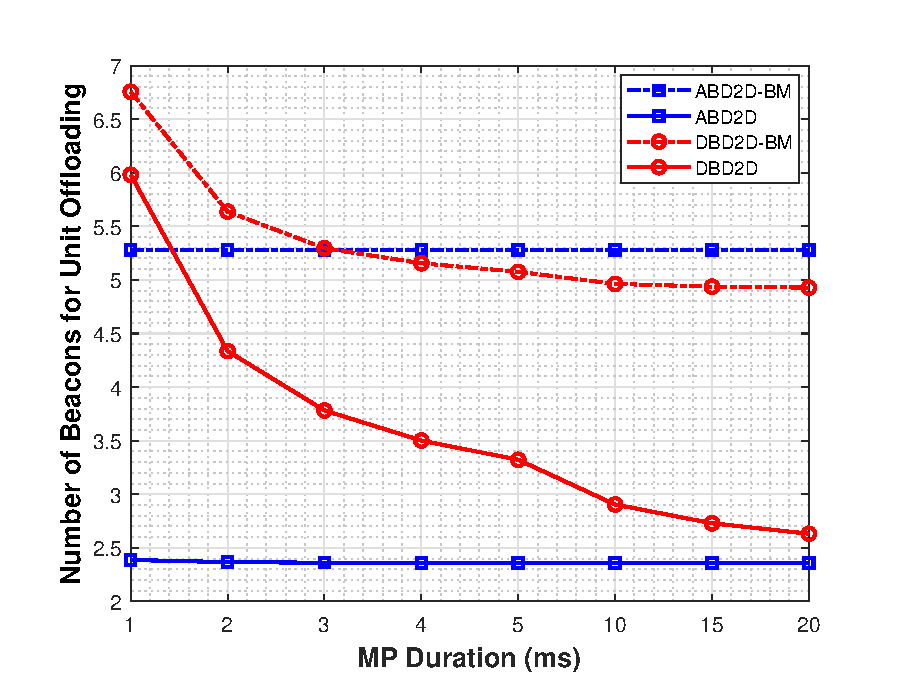
\includegraphics[width=\columnwidth]{MPdur1.eps}
	\caption{Mean number of beacons for unit offloading for varying MP duration}
	\label{fig:MPdur1}
\end{figure}

\begin{figure}[!htb]
	\centering
	
	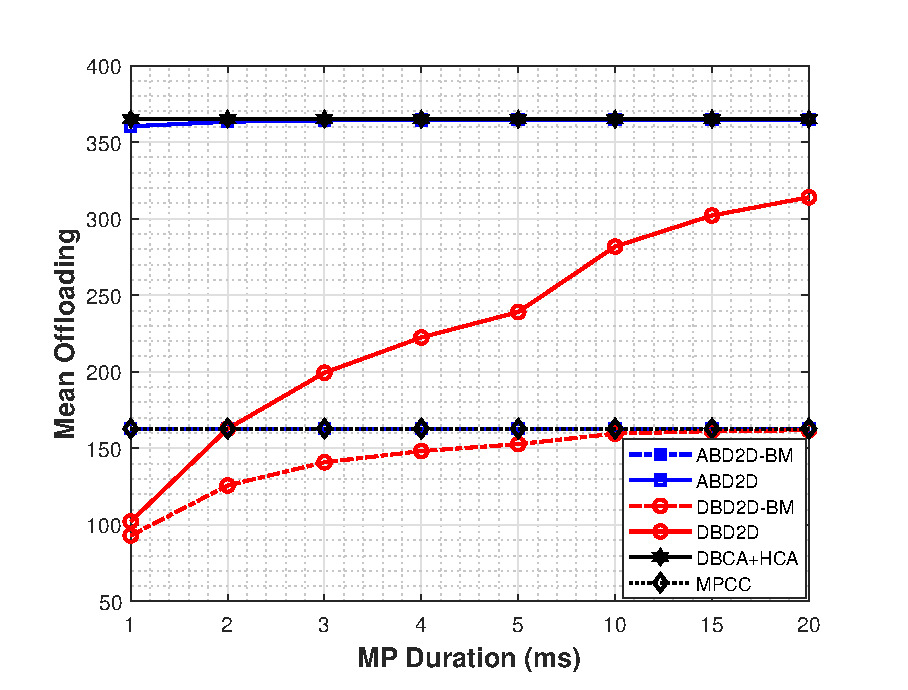
\includegraphics[width=\columnwidth]{MPdur2.eps}
	\caption{Mean offloading for varying MP duration}
	\label{fig:MPdur2}
\end{figure}

Fig. \ref{fig:MPdur1} shows the average number of transmitted beacon messages per successful content offloading as a function of MP duration. Especially for the DBD2D procedure, it is clear that a long MP duration leads to successful discovery attempts and fewer beacon messages are required for successful offloading. On the other hand, for the ABD2D procedure the number of beacons tend to stay stable, though there is a 20-fold increase of the MP duration. The reason for such a tendency is the adequately allocated RBs. A 1 ms long MP provides 10 RBs and thanks to clustering it is enough for 60 HUs, since only CHs transmit the advertisement beacons.



Fig. \ref{fig:MPdur2} is the average offloading for varying MP durations. The offloading performance of the ABD2D procedure looks promising in both latency and offloading. It performs identically to DBCA+HCA for MP duration longer than $2$ ms. On the other hand, for DBD2D even $20$ ms is inadequate for convergence. The large difference ($\approx 200$ units) between ABD2D and ABD2D-BM and MPCC is due to clustering and cache placement in ABD2D.

\begin{figure}[!htb]
	\centering
	
	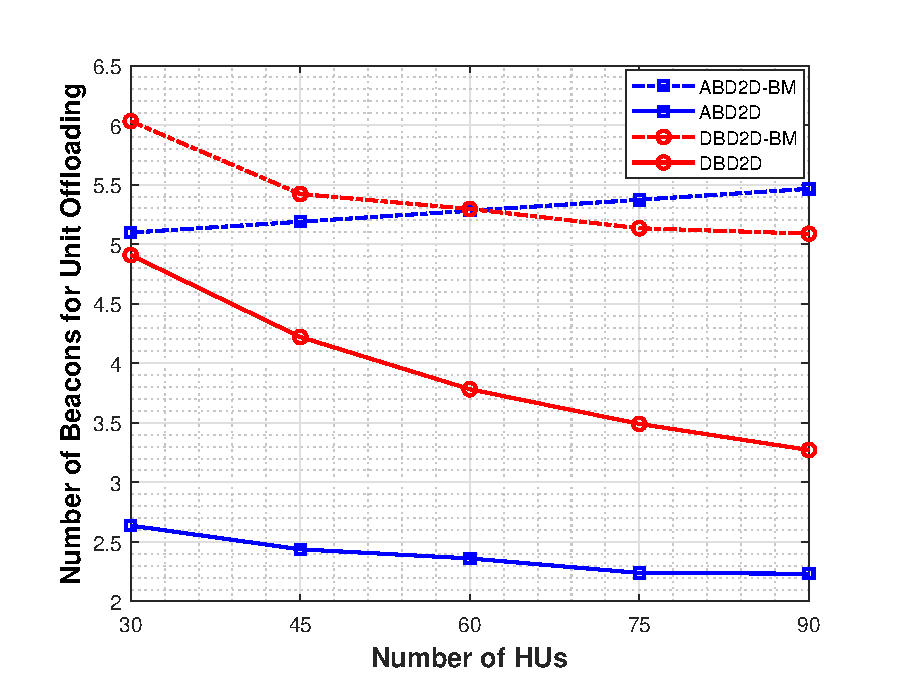
\includegraphics[width=\columnwidth]{H1.eps}
	\caption{Mean number of beacons for unit offloading for different number of HUs}
	\label{fig:H1}
\end{figure}


\begin{figure}[!htb]
	\centering
	
	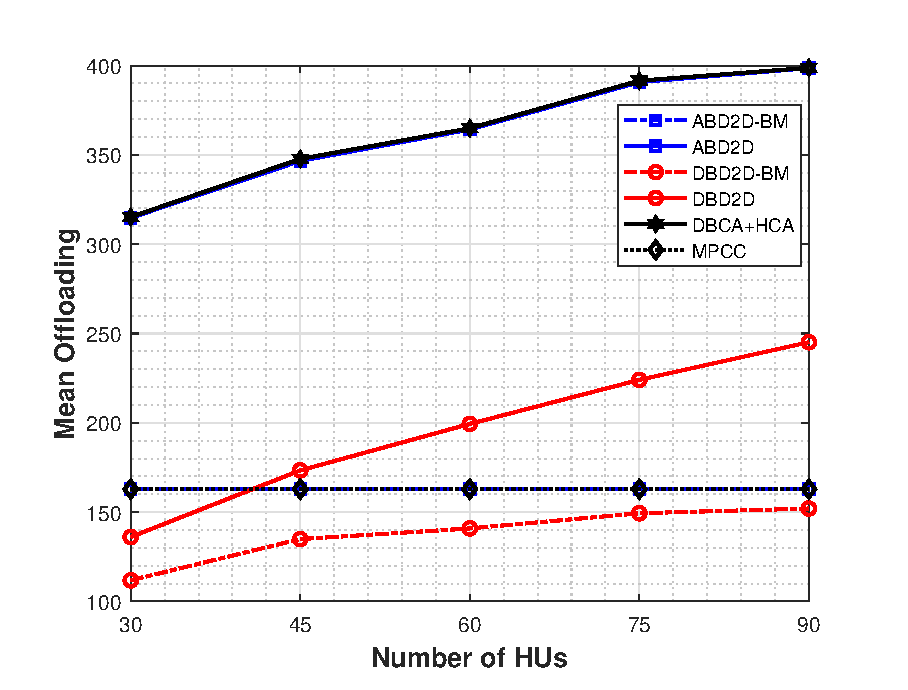
\includegraphics[width=\columnwidth]{H2.eps}
	\caption{Mean offloading for different number of HUs}
	\label{fig:H2}
\end{figure}
Fig. \ref{fig:H1} and Fig. \ref{fig:H2} show the performance of the proposed procedures and benchmark schemes against a varying number of HUs. Plots indicate that increasing number of HUs triggers better offloading except for MPCC and ABD2D-BM since they reach the limit offloading for number of existing OUs. In addition, increase in the offloading amount for ABD2D, DBD2D and DBD2D-BM overcomes the increase in the number of beacons.

\begin{figure}[!htb]
	\centering
	
	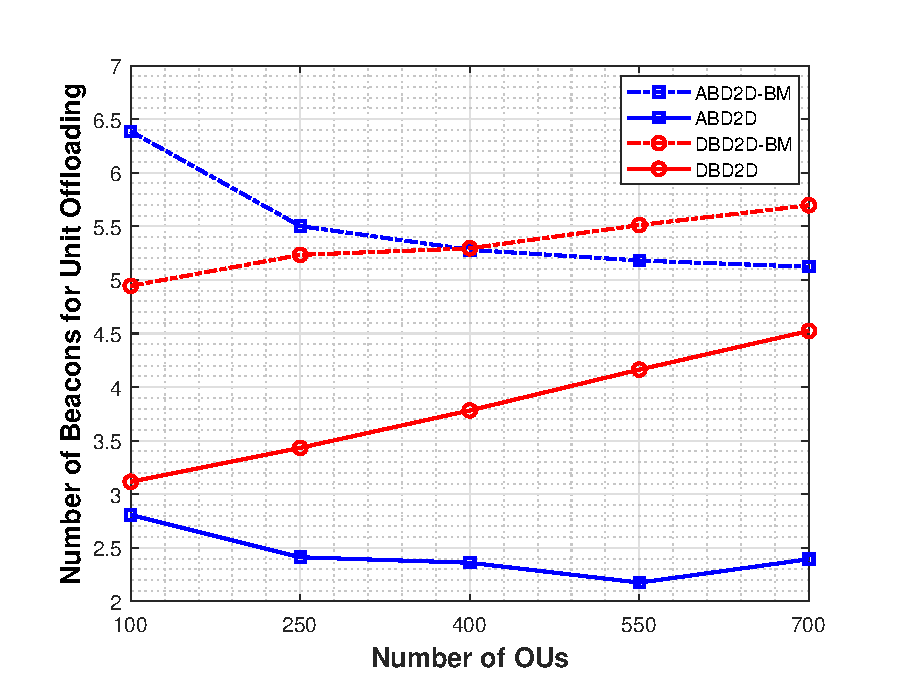
\includegraphics[width=\columnwidth]{OU1.eps}
	\caption{Mean number of beacons for unit offloading for different number of OUs}
	\label{fig:O1}
\end{figure}


\begin{figure}[!htb]
	\centering
	
	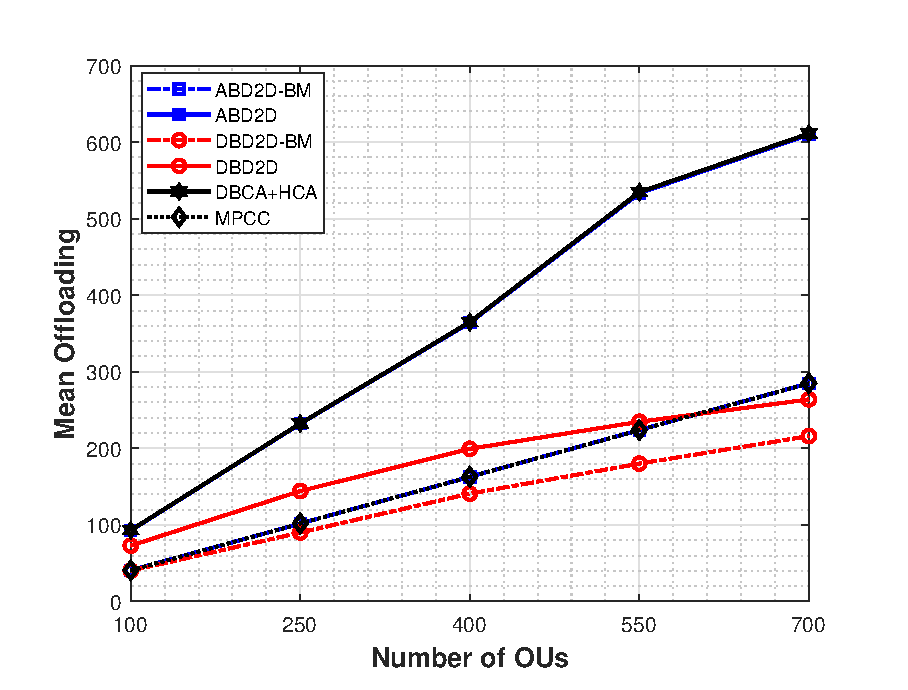
\includegraphics[width=\columnwidth]{OU2.eps}
	\caption{Mean offloading for different number Of OUs}
	\label{fig:O2}
\end{figure}

Fig. \ref{fig:O1} and Fig. \ref{fig:O2} show the average number of beacon messages transmitted per offloaded content for the varying number of OUs.  It is seen that all of the schemes provide better offloading with the increasing number of OUs. This is because each OU increases the data volume of the model network and data demand. For advertisement-based schemes, this increase overcomes the messaging overhead. ABD2D performs almost identically to benchmark DBCA+HCA. This is because only the CHs are designated to initiate content discovery, which decreases collisions and improves offloading. 

\begin{figure}[!htb]
	\centering
	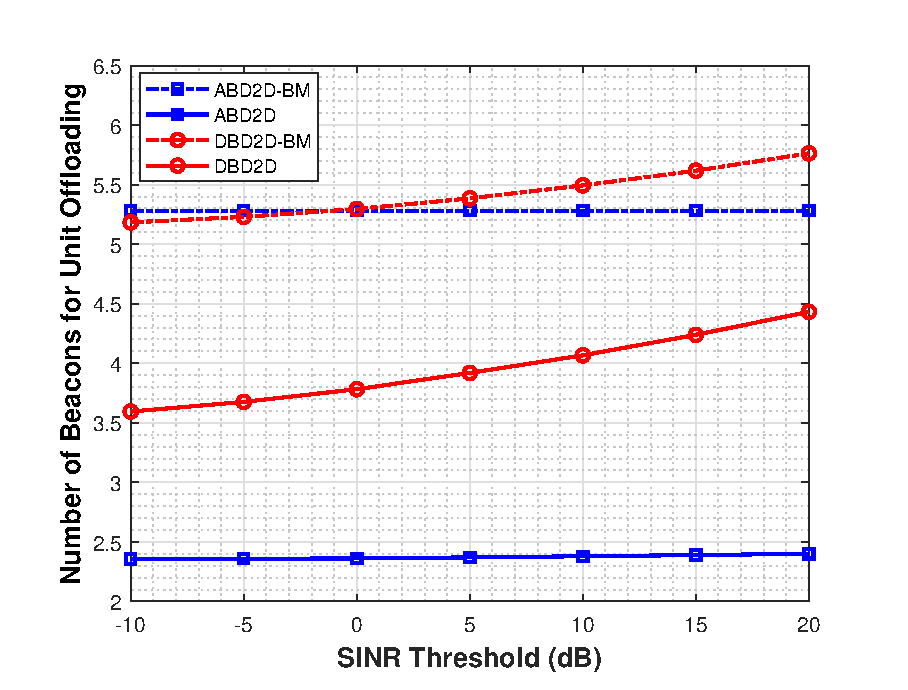
\includegraphics[width=\columnwidth]{SINR1.eps}
	\caption{Mean Number of Beacons for Unit Offloading for Varying SINR Threshold Value}
	\label{fig:SINR1}
\end{figure}


\begin{figure}[!htb]
	\centering
	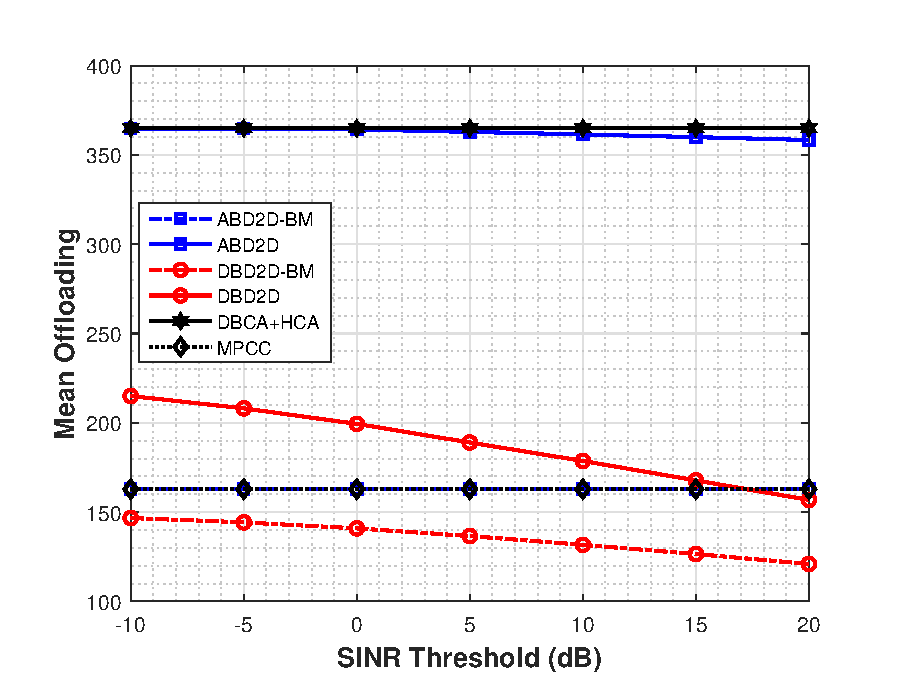
\includegraphics[width=\columnwidth]{SINR2.eps}
	\caption{Mean Offloading for Varying SINR Threshold Value}
	\label{fig:SINR2}
\end{figure}

Lastly, Figs.  \ref{fig:SINR1} and \ref{fig:SINR2} present the performance indicators against varying numbers of SINR threshold. Offloading performance of the proposed ABD2D procedure tends to furcate from the upper bound with the increase in the threshold value. But it is still less than 5\% close to the DBCA+HCA and significantly better than the ABD2D-BM, DBD2D, and DBD2D-BM. Since the number of users does not change, a decrease in the offloading also causes an increase in the number of beacons. These results indicate that the ABD2D procedure is more convenient even for higher-order modulation techniques that require higher SINR values.

\section{Conclusions}
\label{sec:sec7}
In this work, we proposed procedures for Device-to-Device (D2D) cache management, discovery, advertisement, and content delivery. We considered two distinct procedures for device and content discovery and apply them with previously proposed clustering and cache placement algorithms. In the advertisement based scheme (ABD2D) Help Users (HUs) advertise cached content and Ordinary Users (OUs) look for content over a limited number of dedicated resource blocks (RBs). On the other hand, in the discovery based scheme (DBD2D), Ordinary Users (OUs) send discovery messages in order to express to the HUs their need for content.

In both cases, HUs have a clustered structure, which improves both cache placement and content delivery.  For both procedures, we make comprehensive simulations for various performance metrics and against varying parameters. Simulation results show that ABD2D along with clustered HUs, provides less overhead, reduced latency, and improves offloading performance even for compelling circumstances, such as, high user density, less number of dedicated RBs, and high SINR requirement.

In the scope of this paper, we have assumed that the content popularity among users is time-invariant, well known and not user dependent. In a more realistic scenario, stationary and totally identical user preferences are not expected. Therefore, HU-side time-varying popularity and its estimation is planned to be investigated in future work. Furthermore, the attitude of the proposed procedures against mobility will be examined in detail later on in conjunction with cluster lifetime estimation and adaptive clustering and cache placement renewal period. Also the  proposed model and methods for in-band D2D communication must be applicable to existing and future technologies. The LTE Direct framework is considered while deriving a proposed resource allocation model and access methodology. On the other hand, technical reports and specification documents prepared by the 3GPP that cover 5G proximity services are not available yet. Accordingly, adaptation of the network model and proposed methodologies to 5G technology is prioritized for upcoming research.


\printbibliography

\pagebreak

\section*{Authors}
\label{sec:auth}

\begin{wrapfigure}{l}{0.32\columnwidth} 
	\vspace{-.1in}
	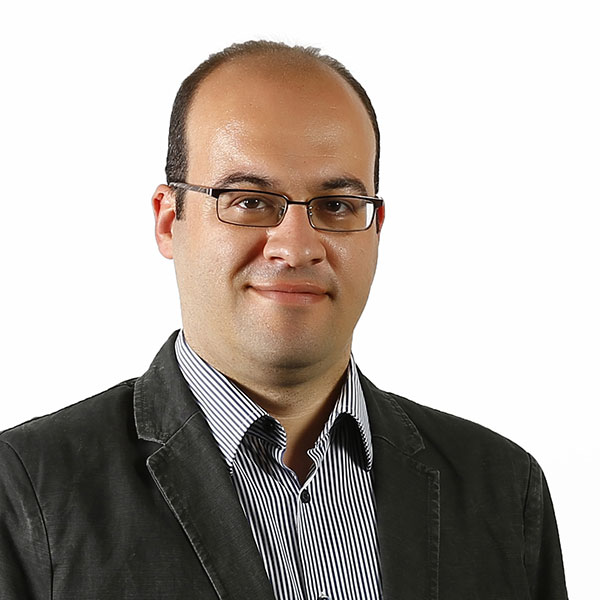
\includegraphics[width=0.37\columnwidth]{tolgagirici.jpg} 
\end{wrapfigure}\textbf{Tolga Girici} received his B.S. degree from Middle East Technical University, Ankara, Turkey in 2000 and Ph.D. degree from University of Maryland, College Park in 2007, both in Electrical Engineering. In 2005, he has spent six months as an intern at the Intelligent Automation Inc, Rockville, MD USA. He was a research assistant at the Fujitsu Labs, College Park MD USA in 2006-2007. He is currently an associate professor at TOBB University of Economics and Technology, Ankara, Turkey. He received a TUBITAK Career Award in 2010, and actively collaborates with industry. His research interests include resource allocation and optimization in next generation cellular wireless access networks, wireless ad hoc networks, smart grid and tactical networks.


\begin{wrapfigure}{l}{0.32\columnwidth} 
	\vspace{-.1in}
	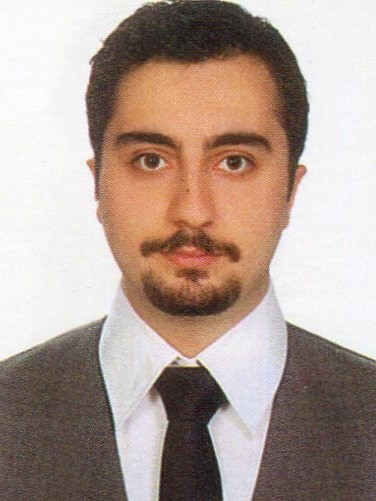
\includegraphics[width=0.32\columnwidth]{ACKazez.jpg} 
\end{wrapfigure}\textbf{Ahmet Cihat Kazez} received his B.S. degree in Electrical and Electronics Engineering from Bilkent University in 2011. He received his M.S. degree in Electrical and Electronics Engineering from TOBB University of Economics and Technology in 2013. He is currently a PhD candidate at the same university. His research interests are routing, scheduling, resource allocation and D2D communications in wireless networks.



\end{document}
